\begin{figure}[h]
    \centering
    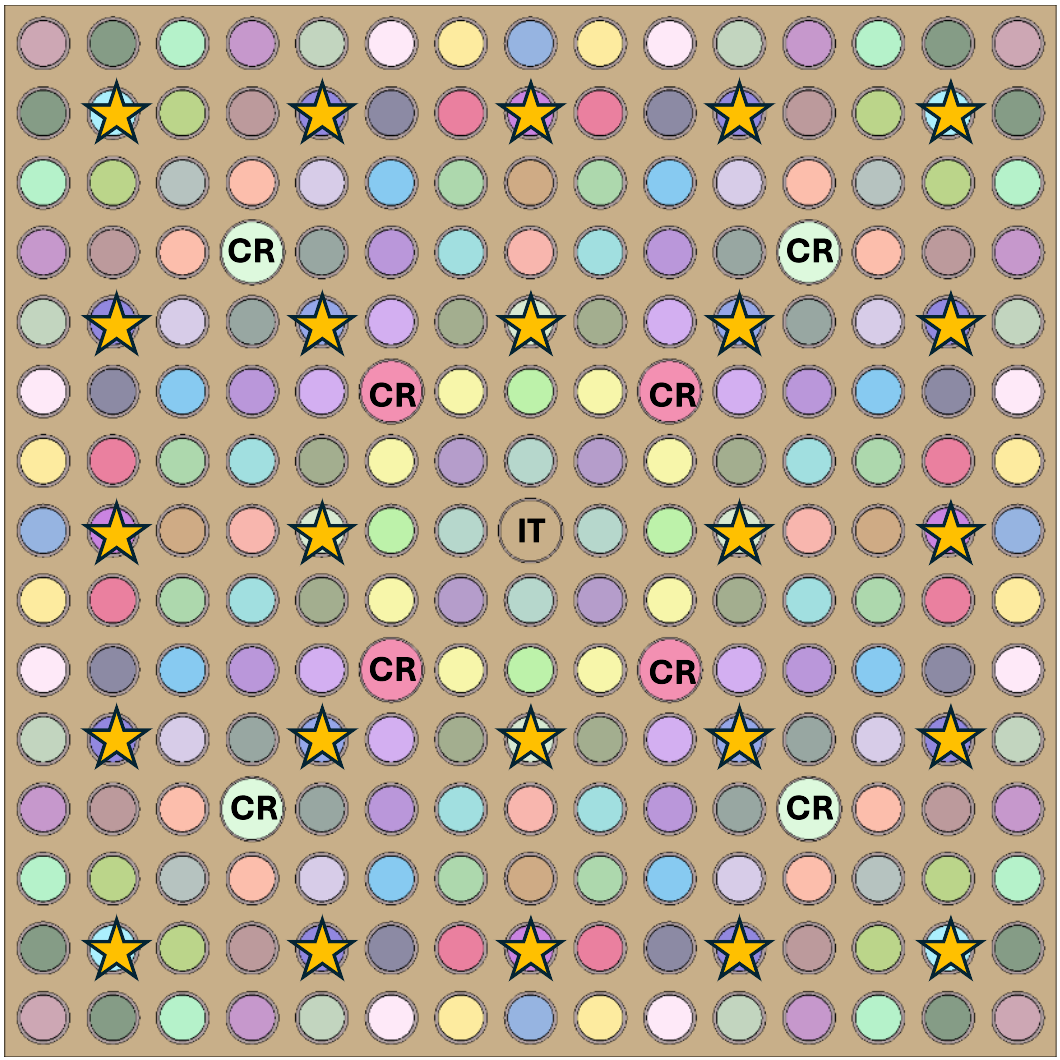
\includegraphics[width=0.5\linewidth]{appendices/CoreLayout.png}
    \caption{Cross section of the assembly layout. The stars show the positions of the power inverter devices, rods labeled \textit{CR} are control rods, and \textit{IT} is an instrumentation tube.}
    \label{fig:placeholder}
\end{figure}


\begin{figure}[H]
    \centering
    \begin{subfigure}[t]{0.48\linewidth}
        \centering
        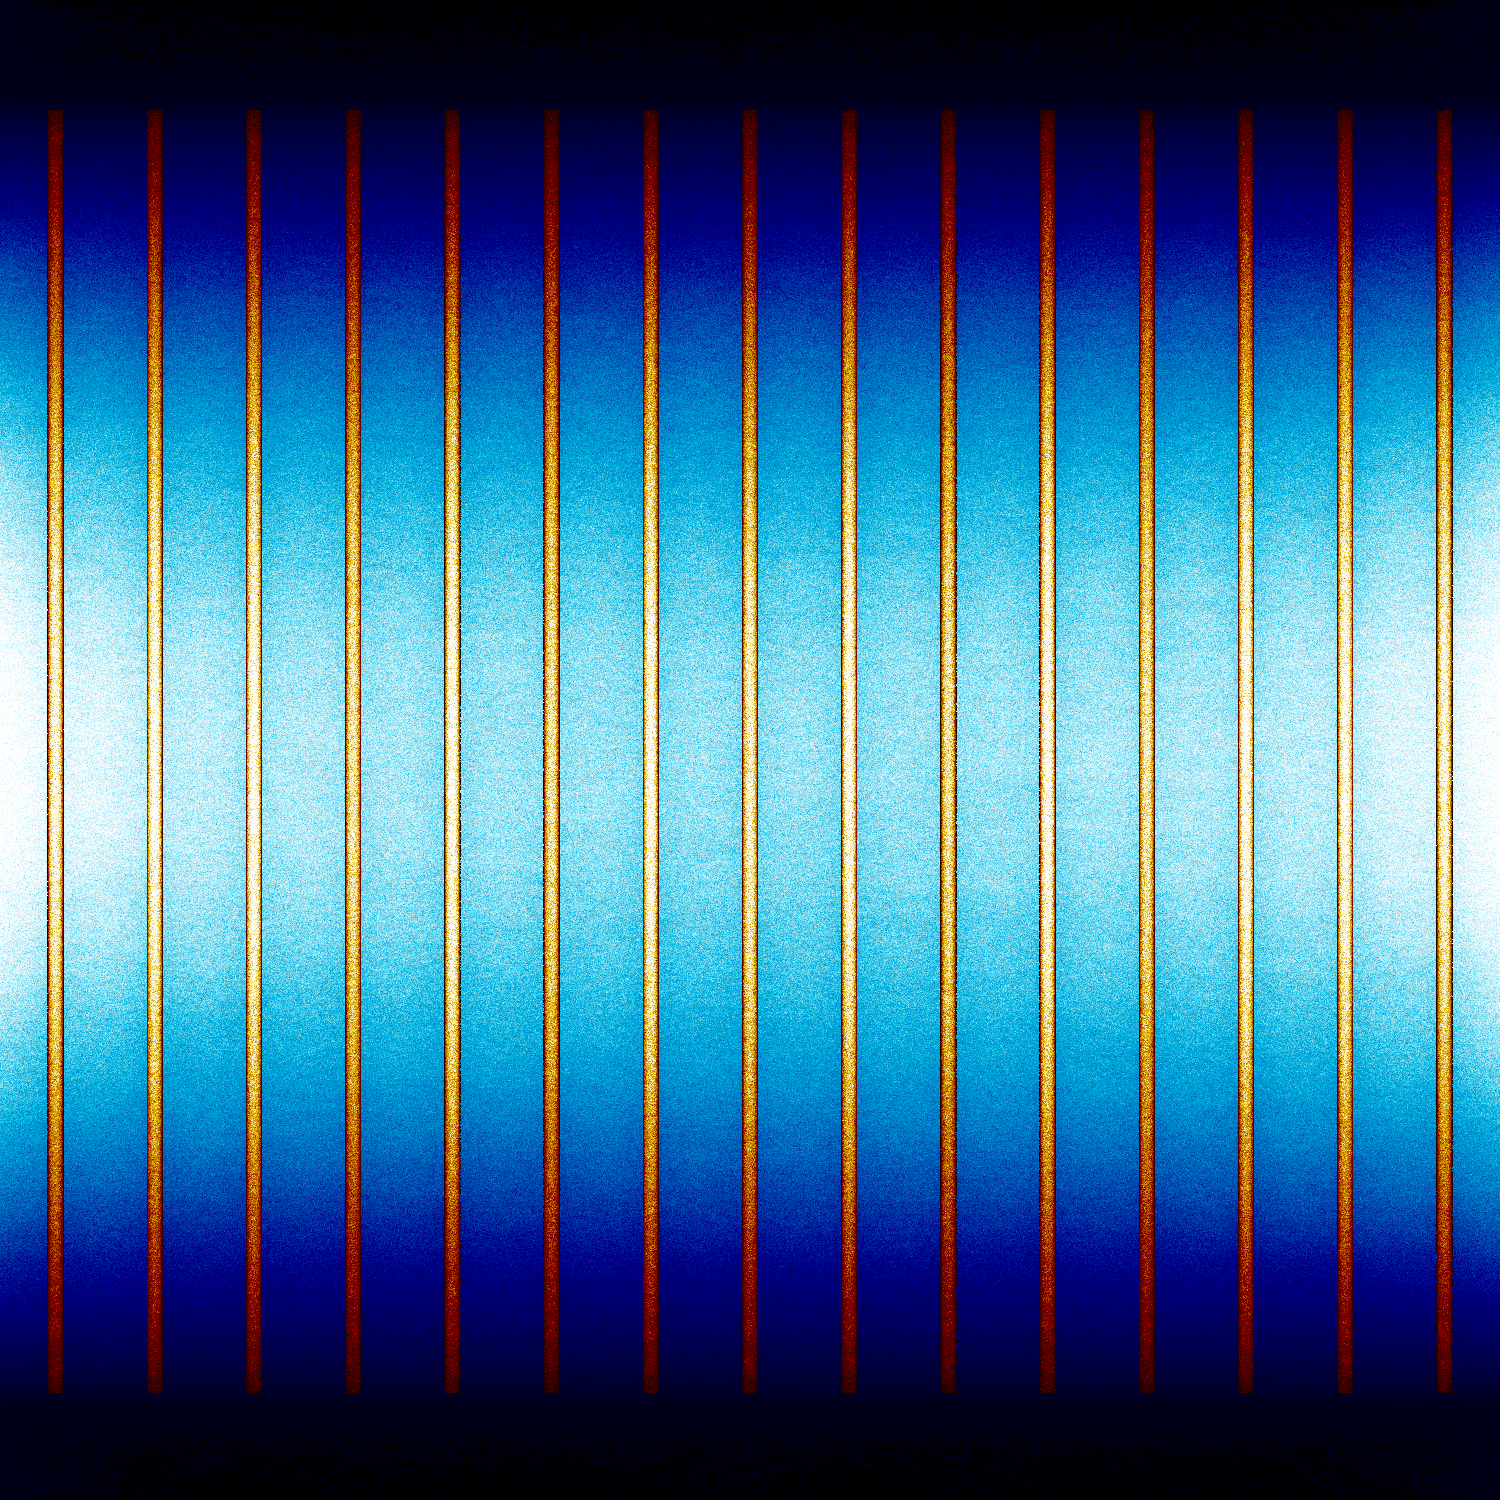
\includegraphics[width=\linewidth]{figs/powerdist-donothing.png}
        \caption{Baseline --- cosine-shaped power profile peaked at the axial midplane, with reduced flux at the rod extremities due to neutron leakage.}
        \label{fig:powerdist_baseline}
    \end{subfigure}
    \hfill
    \begin{subfigure}[t]{0.48\linewidth}
        \centering
        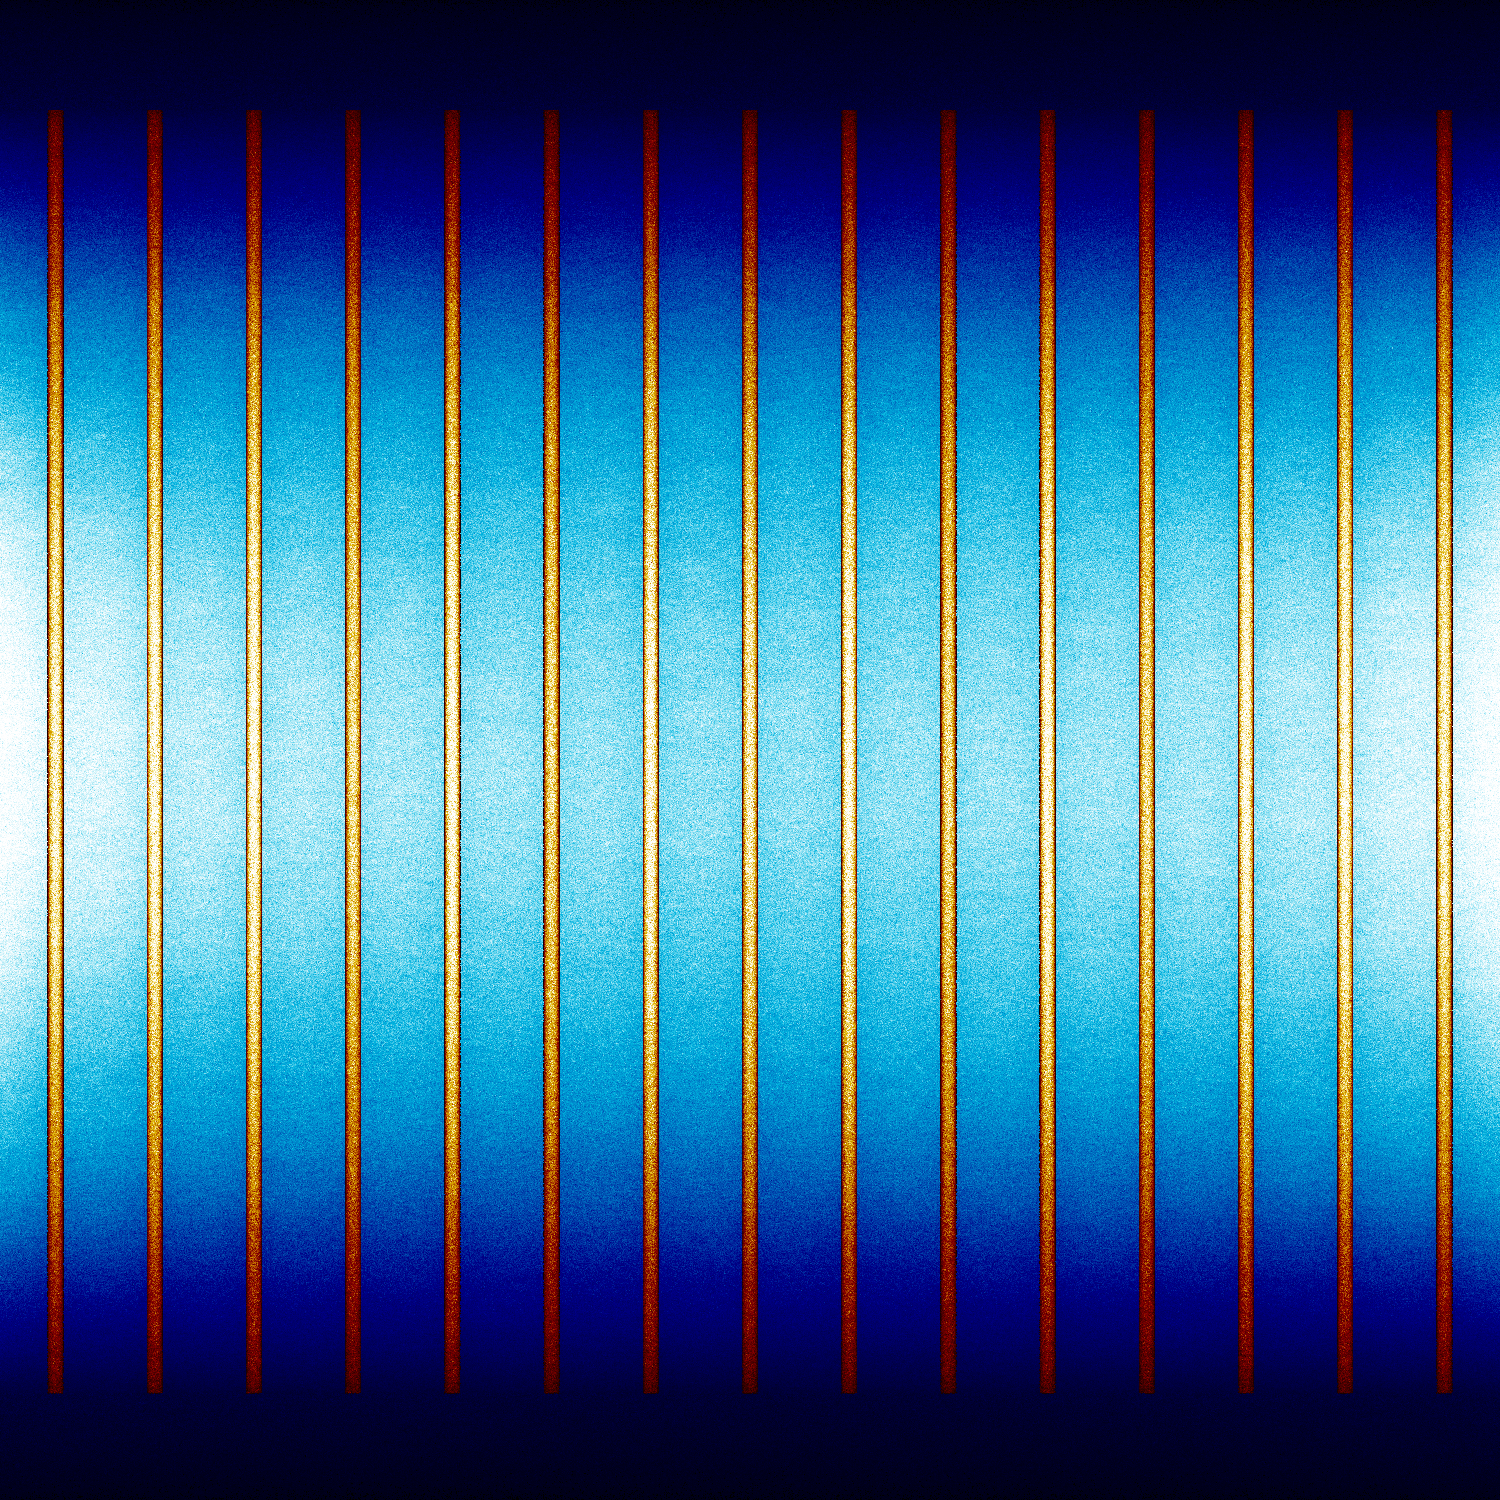
\includegraphics[width=\linewidth]{figs/powerdist-becaps.png}
        \caption{Beryllium End Reflectors --- minimal redistribution relative to the baseline; the cosine shape is largely preserved, indicating limited effectiveness of passive end-reflection.}
        \label{fig:powerdist_becaps}
    \end{subfigure}

    \medskip

    \begin{subfigure}[t]{0.48\linewidth}
        \centering
        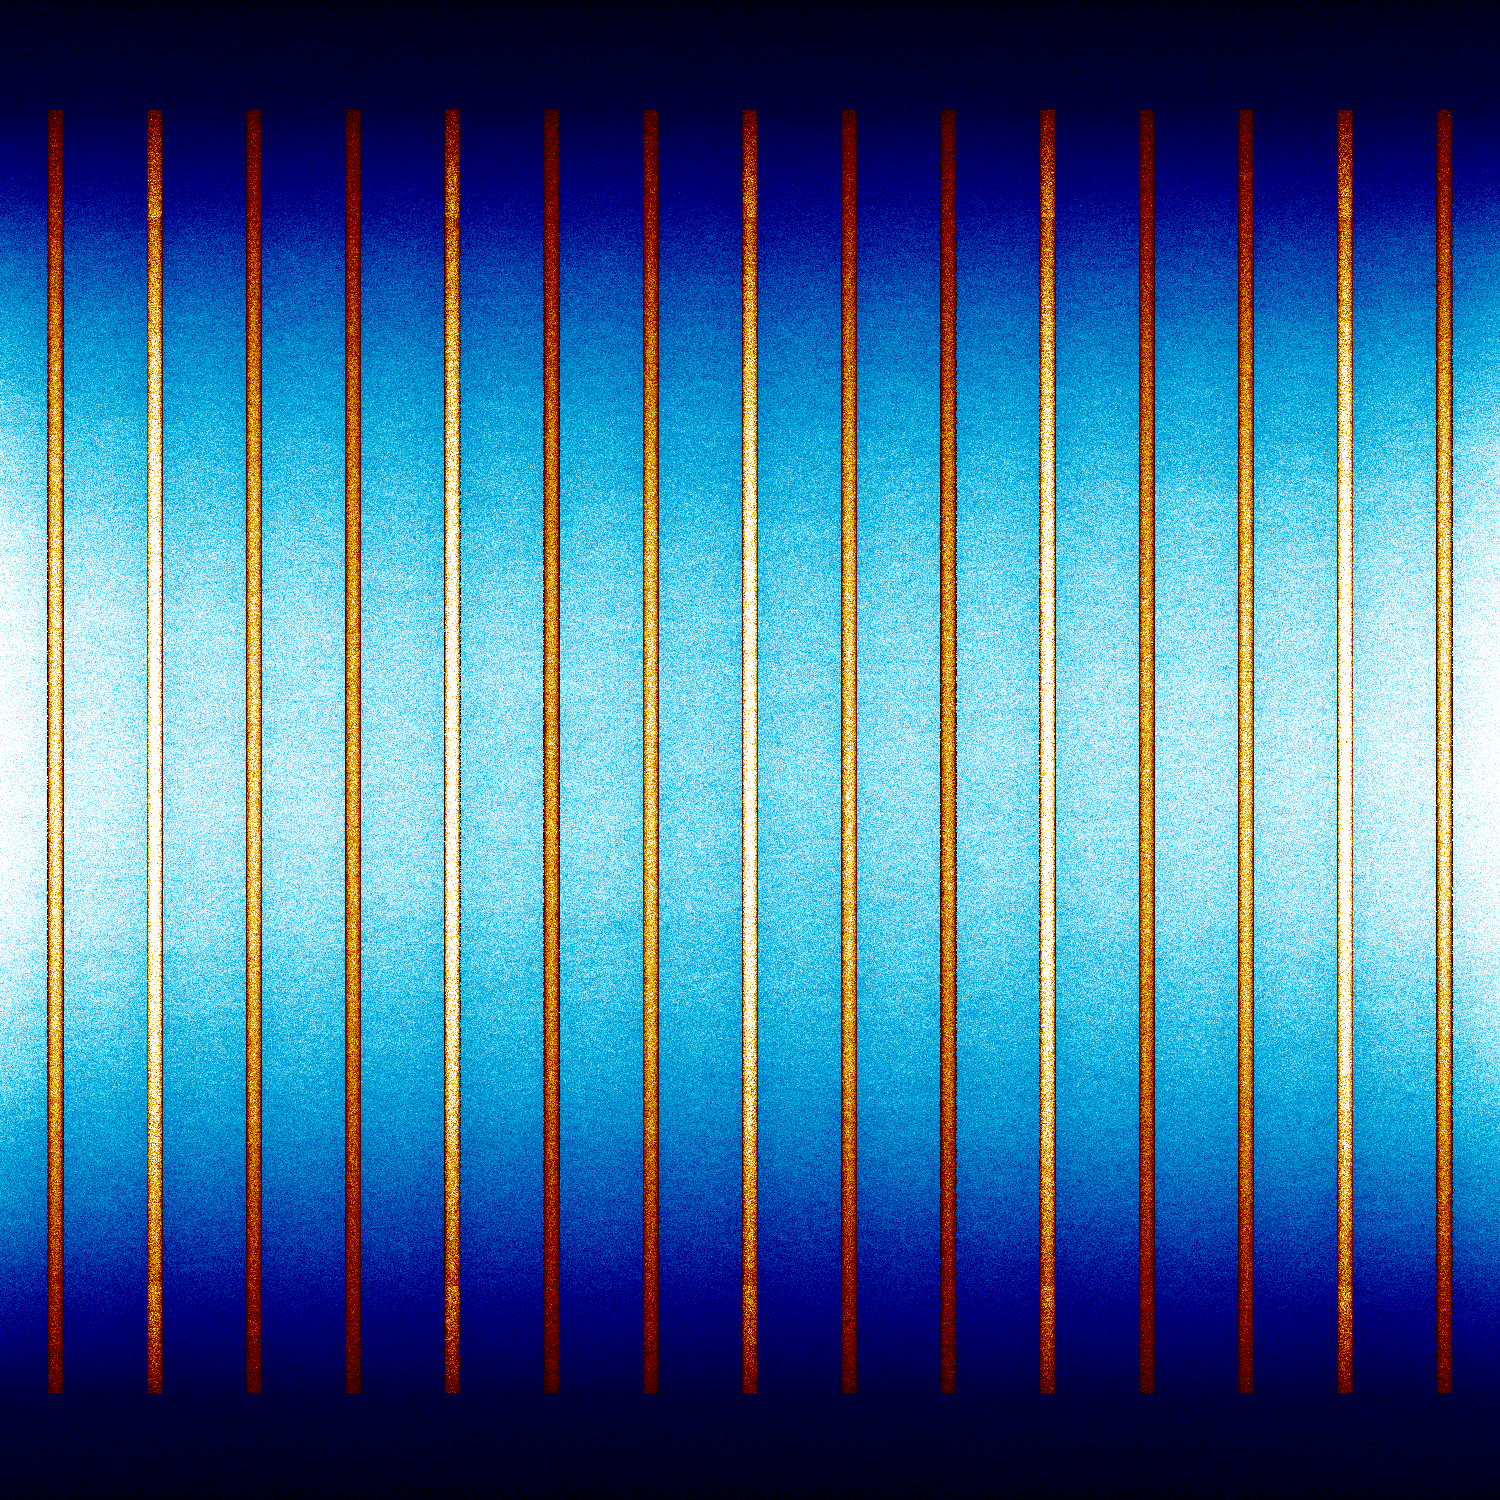
\includegraphics[width=\linewidth]{figs/powerdist-freshrods.png}
        \caption{Fresh Fuel Rods --- elevated and asymmetric power distribution driven by the graded enrichment of the interleaved fresh rods; power remains center-heavy with a shifted axial profile.}
        \label{fig:powerdist_freshrods}
    \end{subfigure}
    \hfill
    \begin{subfigure}[t]{0.48\linewidth}
        \centering
        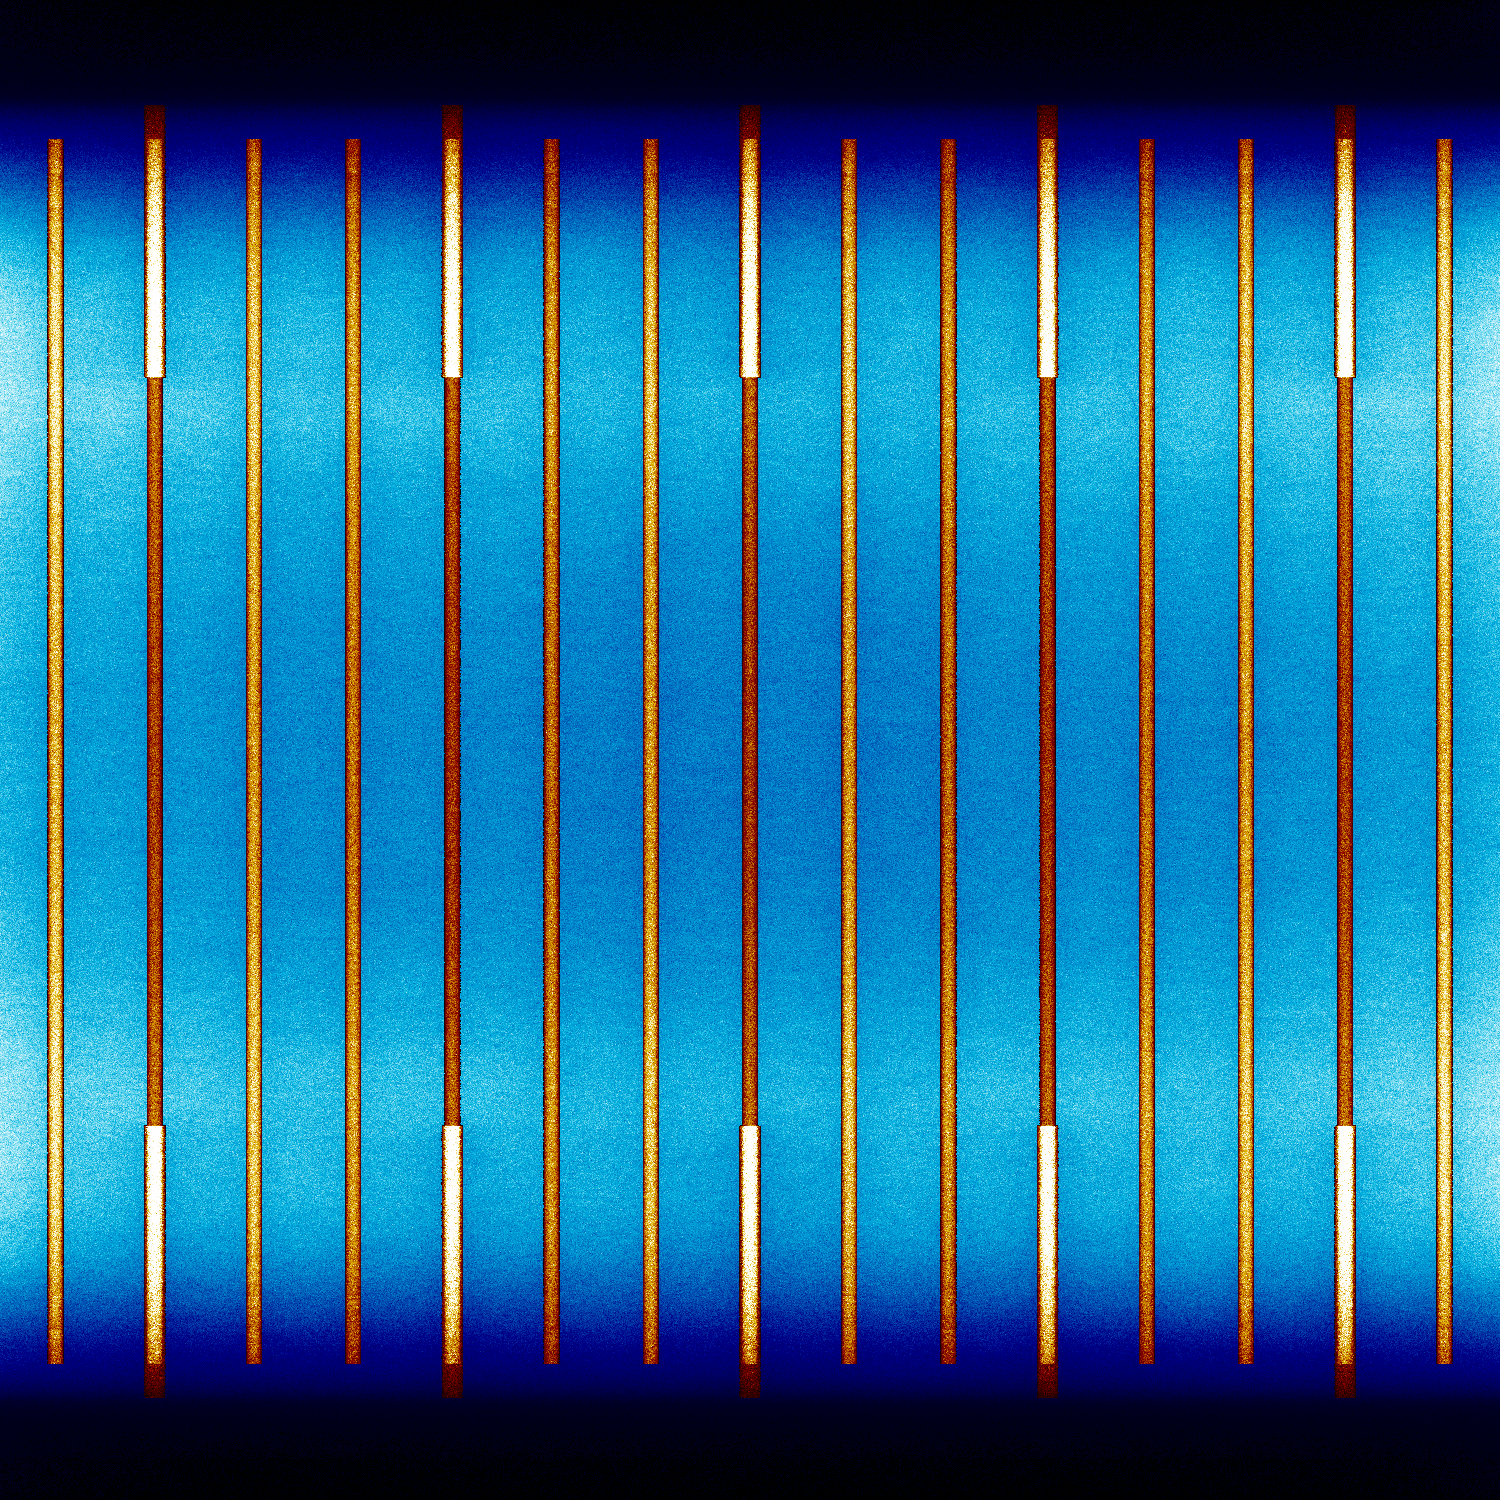
\includegraphics[width=\linewidth]{figs/powerdist-powerinverter.png}
        \caption{Power Inverter Device --- distinctly inverted power profile. The UO$_2$ end regions of the Power Inverter rods produce localized high-flux zones at the axial extremities, while the CeO$_2$ central region yields a dark (low-power) band in the core midplane.}
        \label{fig:powerdist_powerinverter}
    \end{subfigure}

    \caption{Axial power distribution maps for each design variant, rendered as Serpent flux tallies over the assembly cross-section. Brighter color indicates higher local neutron flux and power density. Each image is normalized independently.}
    \label{fig:power_dist_all}
\end{figure}


